\documentclass[11pt]{article}

\usepackage[margin=1in]{geometry}
\usepackage[T1]{fontenc}
\usepackage{lmodern}
\usepackage{amsmath}
\usepackage{booktabs}
\usepackage{graphicx}
\usepackage{longtable}
\usepackage{tocloft}
\usepackage[hidelinks]{hyperref}
\usepackage{etoolbox}
\usepackage{tikz}
\usepackage{pgfplots}

\graphicspath{{assets/}{./}}

\pgfplotsset{compat=1.18}

\setlength{\parindent}{0pt}
\setlength{\parskip}{0.75\baselineskip}

% Dotted leaders in the table of contents
\renewcommand{\cftsecleader}{\cftdotfill{\cftdotsep}}

\title{CO 370 Winter 2026: Group Project Formulation}
\author{
Sa'ad Farooq\thanks{\texttt{s4farooq@uwaterloo.ca}} \and
Maxwell Fang\thanks{\texttt{m34fang@uwaterloo.ca}} \and
Buck Chen\thanks{\texttt{b39chen@uwaterloo.ca}} \and
Timothy Zheng\thanks{\texttt{t54zheng@uwaterloo.ca}}
}

\begin{document}
\maketitle
\vspace{-1.75em}

\section{Topic}
\begin{center}
Optimal Power Flow (Direct Current Approximation)
\end{center}

\begin{abstract}
The North American electricity grid operates as a market on a nodal network of energy ``settlement points'' connected by capacity-constrained transmission lines. Participants are generators (gens) and loads, which buy and sell power through an auction process.

The role of the grid operator (RTO) is to ensure economic dispatch of power through a clearing process that tells gens and loads how much power they are allowed (or obligated) to deposit or withdraw from the grid at each settlement point at any given time. 

Since electricity cannot be easily stored, it is instantly delivered across power lines. To effectively manage the supply and demand characteristics in the market, a production/usage schedule is generated which ensures that power lines are not overloaded. This schedule is generated under a constrained linear program which maximizes for the total amount of power being transmitted while subject to power line limit constraints and bid/ask prices from power supplies and users. Once cleared, all market participants are obligated to generate or consume their scheduled amount of electricity to maintain grid stability. Participants must buy or sell in a seperate, lower supply and therefore higher priced real-time market if they are unable to meet their obligations to make their positions whole. In the realtime market, production schedules are computed every five minutes, making the efficient execution of power calculations necessary. Due to the limit in transmission capacity across power lines, power prices tend to be different in different geographical regions, and can be deterministically calculated through LP. 

This report is a recreation of the end-to-end process of running the scheduling calculation done by the RTO. Moreover, we also aim to, as an extension, clear one simulated auction round in the electricity derivatives market for a product called Financial Transmission Rights (FTR). We believe this project is highly relevant given the rapid rise of electricity demand from data centers and manufacturing, and the rise of extreme weather that makes key grid elements more sensitive to catastrophic failures that can result in blackouts.
\end{abstract}

\newpage
\tableofcontents
\newpage

% ----------- Problem Description ---------------
\section{Problem Description}

In summary, market participants submit bids (loads) and offers (gens) for power by specifying the (1) amount, (2) price per MWh, and (3) node where electricity is demanded. The goal of this project is to determine the optimal solution given these bids and offers to generate a production schedule which economically solves this auction (maximal power is transacted while adhering to bid and offer prices) while also adhering to transmission limit constraints. 

To describe the problem, here is a motivating 3-node grid.

\begin{minipage}[t]{0.40\textwidth}
    \begin{center}
    \resizebox{\linewidth}{!}{%
    \begin{tikzpicture}[every node/.style={font=\normalsize}]
        \node[draw, circle, minimum size=1.2cm] (A) at (0,2.8) {A};
        \node[draw, circle, minimum size=1.2cm] (B) at (6.6,2.8) {B};
        \node[draw, circle, minimum size=1.2cm] (C) at (3.3,0) {C};

        \draw[thick] (A) -- (B);
        \draw[thick] (B) -- (C);
        \draw[thick] (A) -- (C);

        \node[align=left] at (-2.3,2.9) {Gen 1\\Load 1};
        \node[align=left] at (8.8,2.9) {Gen 2};
        \node[align=center] at (3.3,-1.4) {Gen 3\\Load 2, Load 3};
    \end{tikzpicture}%
    }
    \end{center}

    \vspace{0.5em}
    \textbf{Line limits}
    \begin{center}
    \scriptsize
    \resizebox{0.9\linewidth}{!}{%
    \begin{tabular}{lc}
        \toprule
        Line & Limit \\
        \midrule
        $A \rightarrow C$ & 3 MW \\
        $A \rightarrow B$ & 3 MW \\
        $B \rightarrow C$ & 3 MW \\
        \bottomrule
    \end{tabular}%
    }
    \end{center}
\end{minipage}\hfill
\begin{minipage}[t]{0.56\textwidth}
    \textbf{Supply offers}
    \begin{center}
    \scriptsize
    \resizebox{\linewidth}{!}{%
    \begin{tabular}{lccc}
        \toprule
        Generator & Node & Offer & Max MW \\
        \midrule
        Gen 1 & $A$ & \$5.00 & 2.0 \\
        Gen 2 & $B$ & \$10.00 & 10.0 \\
        Gen 3 & $C$ & \$7.50 & 0.5 \\
        \bottomrule
    \end{tabular}%
    }
    \end{center}

    \vspace{0.4em}
    \textbf{Demand bids}
    \begin{center}
    \scriptsize
    \resizebox{\linewidth}{!}{%
    \begin{tabular}{lccc}
        \toprule
        Load & Node & Demand & Bid \\
        \midrule
        Load 1 & $A$ & 1.0 & \$6.50 \\
        Load 2 & $C$ & 2.0 & \$7.50 \\
        Load 3 & $C$ & 1.5 & \$10.00 \\
        \bottomrule
    \end{tabular}%
    }
    \end{center}
\end{minipage}

\subsection{Bids and Offers}
In an auction selling multiple units of a commodity with no differentiation, such as power at a certain node $i$, the auction clearing process determines a price point $P_i$ where the maximum monetary value of power is transacted, while ensuring the sum of capacity bid by loads bidding over $P_i$ is equal to the sum of capacity offered by gens offering at prices under or equal to $P_i$. Once determined, all participants buy and sell at that one price. This style of auction is known as a \textit{Dutch Auction}, which has good properties for a constrained clearing process outlined below.

\newpage
Suppose the market clearing process determines the following feasible solution.

\begin{center}
    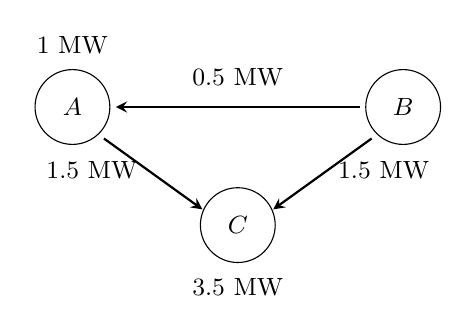
\begin{tikzpicture}[>=stealth, every node/.style={font=\small}]
        \node[draw, circle, minimum size=0.95cm] (A) at (0,1.5) {$A$};
        \node[draw, circle, minimum size=0.95cm] (B) at (4.2,1.5) {$B$};
        \node[draw, circle, minimum size=0.95cm] (C) at (2.1,0) {$C$};

        \node[above] at (0,2.05) {$1$ MW};
        \node[below] at (2.1,-0.55) {$3.5$ MW};

        \draw[->, thick] (3.65,1.5) -- (0.55,1.5);
        \node[above] at (2.1,1.65) {$0.5$ MW};

        \draw[->, thick] (0.4,1.1) -- (1.65,0.2);
        \node[left] at (0.95,0.7) {$1.5$ MW};

        \draw[->, thick] (3.8,1.1) -- (2.55,0.2);
        \node[right] at (3.25,0.7) {$1.5$ MW};
    \end{tikzpicture}
\end{center}

Here, since all bids were above the clearing price at each node, the loads are fully filled. To satisfy this demand, the feasible solution requires that:

\begin{itemize}
    \item Gen 1 produces 2 MW.
    \item Gen 2 produces 2 MW.
    \item Gen 3 produces 0.5 MW.
\end{itemize}

\subsection{Shift Factors}

Shift factors are critical for the auction clearing process. Shift factors are defined on a per-line basis, and are further parameterized by specifying a $\textit{sink}$ and $\textit{source}$ node. The shift factor is a constant specifying how much of 1MW injected into the grid at the source and then withdrawn from the sink goes through the line. Shift factors are used to calculate the total load on each line for a given production schedule, which solves for the total transmission on each line given each node's net supply/demand.

For example, here are example shift factors in our 3-node grid example.

\textbf{Shift factors for source $A$, sink $C$}

\begin{center}
\begin{tabular}{ccc}
    \toprule
    $A \rightarrow B$ & $B \rightarrow C$ & $A \rightarrow C$ \\
    \midrule
    0.1 & 0.1 & 0.9 \\
    \bottomrule
\end{tabular}
\end{center}

\vspace{0.2em}
1 MW injected at $A$ and withdrawn at $C$ flows as follows:

\begin{center}
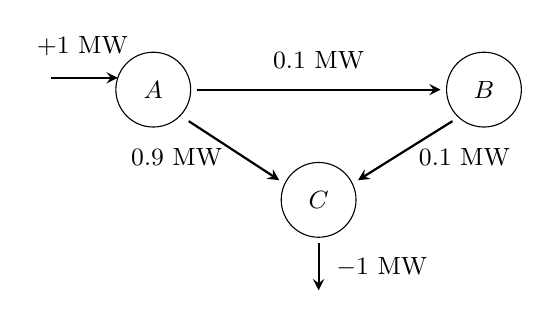
\begin{tikzpicture}[>=stealth, every node/.style={font=\small}]
    \node[draw, circle, minimum size=0.95cm] (A) at (0,1.4) {$A$};
    \node[draw, circle, minimum size=0.95cm] (B) at (4.2,1.4) {$B$};
    \node[draw, circle, minimum size=0.95cm] (C) at (2.1,0) {$C$};

    \draw[->, thick] (-1.3,1.55) -- (-0.45,1.55);
    \node[above] at (-0.9,1.7) {$+1$ MW};

    \draw[->, thick] (0.55,1.4) -- (3.65,1.4);
    \node[above] at (2.1,1.55) {$0.1$ MW};

    \draw[->, thick] (0.45,1.0) -- (1.6,0.25);
    \node[left] at (1.0,0.55) {$0.9$ MW};

    \draw[->, thick] (3.8,1.0) -- (2.6,0.25);
    \node[right] at (3.25,0.55) {$0.1$ MW};

    \draw[->, thick] (2.1,-0.55) -- (2.1,-1.15);
    \node[right] at (2.2,-0.85) {$-1$ MW};
\end{tikzpicture}
\end{center}

\newpage

\subsection{(N-1) Security Constraint}

In addition to the above restrictions, the grid operator imposes a \textit{(N-1) Contingency Analysis}, which ensures that any feasible production schedule is also feasible all grids where one line goes offline. This ensures grid reliability since unpredicted outages can happen for many reasons such as safety concerns, weather, or unexpected damage caused by accidents or falling trees.

In our 3-node example, the (N-1) contingency analysis looks like this. Note that our proposed solution is feasible in all 3 scenarios, and so this is a valid production schedule that can be sent out to market participants.

\noindent
\begin{minipage}[t]{0.32\textwidth}
    \vspace{0pt}
    \centering
    \textbf{$A \rightarrow B$ down}

    \vspace{0.35em}

    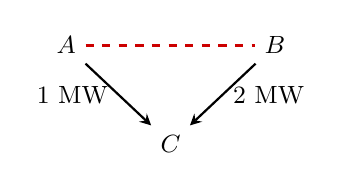
\begin{tikzpicture}[scale=0.78, every node/.style={font=\small}, >=stealth]
        \node (A) at (0,1.6) {$A$};
        \node (B) at (3.4,1.6) {$B$};
        \node (C) at (1.7,0) {$C$};

        \draw[red!80!black, dashed, thick] (A) -- (B);
        \draw[->, thick] (A) -- node[left] {$1$ MW} (C);
        \draw[->, thick] (B) -- node[right] {$2$ MW} (C);
    \end{tikzpicture}
\end{minipage}\hfill
\begin{minipage}[t]{0.32\textwidth}
    \vspace{0pt}
    \centering
    \textbf{$A \rightarrow C$ down}

    \vspace{0.35em}

    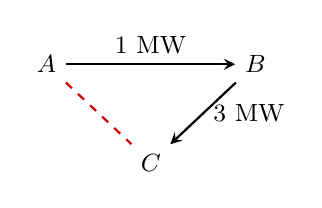
\begin{tikzpicture}[scale=0.78, every node/.style={font=\small}, >=stealth]
        \node (A) at (0,1.6) {$A$};
        \node (B) at (3.4,1.6) {$B$};
        \node (C) at (1.7,0) {$C$};

        \draw[->, thick] (A) -- node[above] {$1$ MW} (B);
        \draw[->, thick] (B) -- node[right] {$3$ MW} (C);
        \draw[red!80!black, dashed, thick] (A) -- (C);
    \end{tikzpicture}
\end{minipage}\hfill
\begin{minipage}[t]{0.32\textwidth}
    \vspace{0pt}
    \centering
    \textbf{$B \rightarrow C$ down}

    \vspace{0.35em}

    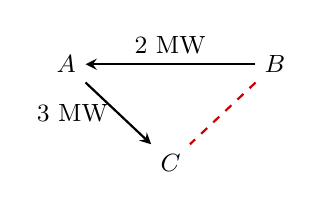
\begin{tikzpicture}[scale=0.78, every node/.style={font=\small}, >=stealth]
        \node (A) at (0,1.6) {$A$};
        \node (B) at (3.4,1.6) {$B$};
        \node (C) at (1.7,0) {$C$};

        \draw[<-, thick] (A) -- node[above] {$2$ MW} (B);
        \draw[->, thick] (A) -- node[left] {$3$ MW} (C);
        \draw[red!80!black, dashed, thick] (B) -- (C);
    \end{tikzpicture}
\end{minipage}

\subsection{Locational Marginal Prices (LMPs)}

Due to capacity limits on power lines, more cost-effective power generators may not be authorized to produce power, despite a load willing to pay high prices for power. In these scenarios, power from a more expensive plant must be dispatched to fulfill the demand, resulting in a higher clearing price at the demand node and resulting in different power prices per region in the grid. The mathematics to determine LMPs are deterministic on the dual variables in the feasible solution in the LP and grid shift factors (aka ``Power Transfer Distribution Factors
`` (PTDF)s). The full calculation is found in $\textbf{Appendix 1}$.

\subsection{Financial Transmission Rights (FTR)}

Financial Transmission Rights (FTR) are derivative contracts\footnote{\url{https://en.wikipedia.org/wiki/Derivative_(finance)}} where the underlying is the congestion between any two nodes $(a, b)$ in a power grid. Their payout is calculated as


$$\text{Payout} = (LMP_{Sink} - LMP_{Source}) \times \text{Quantity (MW)}$$

where the $(LMP_{Sink} - LMP_{Source})$ is known as congestion.

Congestion is only non-zero in the case where constraints in the DA clearance are binding (the inequality replaced with equality).

The trading of these contracts does not affect the underlying power market, however it is a common tool used by market participants to hedge their operations against congestion costs. If the difference is positive, the contract holder is paid by the RTO. If the difference is negative, the contract holder is obligated to pay the RTO the difference. For example, a utility provider may purchase FTRs to guarantee their customers a fixed price for electricity, which is preferred to power prices that fluctuate daily and are unpredictable. Power plants may also purchase these contracts to guarantee a sale price to lock in their profit margins.

\subsection{FTR Clearance}
The clearing process is formally defined in the references in the Iowa State paper (Ma, et al.) As a summary, the FTR clearing process is mostly similar to the DA clearing process however the unit allocation is not bounded by the generation/demand capacity, but instead the amount of bids and offers, ultimately capped by the transmission capacity of a branch. For example, on a line going from node $A \rightarrow B$ with capacity $100\text{MW}$, up to $150\text{MW}$ of capacity can be cleared for that line, given that for the $50\text{MW}$ of excess capacity sold, there are at least $50\text{MW}$ cleared for $B \rightarrow A$.

\textbf{Rationale} (to why net FTR volume over a line is capped by the transmission limit of the line): Note that the shadow price of a line is going to be 0 if it is not binding (the amount of electricity being transmitted is less than the limit). The shadow price is only going to be non-zero if the line is binding, and the capacity is reached.

Since the RTO only needs to pay out (or receive payment) from the derivative in the case where the congestion is non-zero, and congestion on a line is a linear function of the shadow price on the line, the RTO only wants to sell up to the capacity of the line to ensure they can collect the necessary congestion rent from the difference from the DA market.

\textbf{Why is congestion rent positive? } Generators sometimes sell at a lower price at their pricing node, but electricity purchased at another node (suppose this node has no generation) will be more expensive due to demand at a supply-constrained node; then the buyers pay a higher LMP while the seller only receives the cheaper node's LMP. The "profit" generated by the RTO goes straight into paying FTRs.

\subsection{Clearing Process Flowchart}

\begin{center}
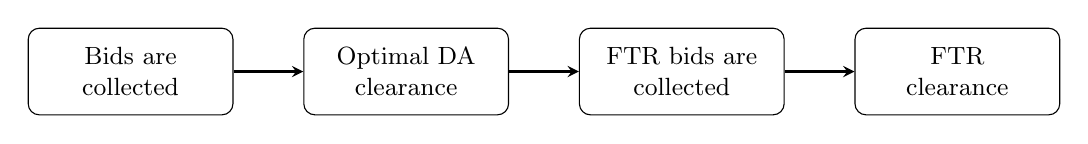
\begin{tikzpicture}[>=stealth, font=\small]
  \node[draw, rounded corners, minimum width=2.6cm, minimum height=1.1cm, align=center] (s1) at (0,0) {Bids are\\collected};
  \node[draw, rounded corners, minimum width=2.6cm, minimum height=1.1cm, align=center] (s2) at (3.5,0) {Optimal DA\\clearance};
  \node[draw, rounded corners, minimum width=2.6cm, minimum height=1.1cm, align=center] (s3) at (7.0,0) {FTR bids are\\collected};
  \node[draw, rounded corners, minimum width=2.6cm, minimum height=1.1cm, align=center] (s4) at (10.5,0) {FTR\\clearance};

  \draw[->, thick] (s1.east) -- (s2.west);
  \draw[->, thick] (s2.east) -- (s3.west);
  \draw[->, thick] (s3.east) -- (s4.west);
\end{tikzpicture}
\end{center}

% ----------- Formulation --------------- 

\section{Formulation}

\subsection{DA Clearance LP Formulation Setup}

Due to the size of these parameters, the definition of each parameter is defined in the appendix, with the full LP described below.

\textbf{LP Objective Function}

\begin{equation}
\max_{g,d} \quad
\sum_{d \in \mathcal{D}} p_d d_d
-
\sum_{g \in \mathcal{G}} c_g g_g
\end{equation}


Defines nodal net injection used to compute transmission flows via PTDFs.

\subsection{Base-Case Transmission Constraints}

\begin{equation}
- F_l^{\max}
\le
\sum_{s \in \mathcal{N}} PTDF_{l,s} \, inj_s
\le
F_l^{\max}
\quad \forall l \in \mathcal{L}
\end{equation}

 
Ensures no transmission line exceeds its thermal rating under normal operating conditions.

\textbf{Contingency Constraints (N-1 Security)}

\begin{equation}
- F_l^{\max}
\le
\sum_{s \in \mathcal{N}} PTDF_{l,s}^{(k)} \, inj_s
\le
F_l^{\max}
\quad \forall l \in \mathcal{L}, \forall k \in \mathcal{K}
\end{equation}

 
Guarantees that the chosen dispatch remains feasible if any single contingency occurs.  
The same generation dispatch must satisfy all contingency flow limits (no corrective redispatch).

\subsection{Full DA Market Clearing Formulation}

\begin{align}
\max_{g,d} \quad
& \sum_{d \in \mathcal{D}} p_d d_d
- \sum_{g \in \mathcal{G}} c_g g_g
\\[6pt]
\text{s.t.} \quad
& \sum_{g \in \mathcal{G}} g_g
-
\sum_{d \in \mathcal{D}} d_d
= 0
\\[6pt]
& g_g^{\min} \le g_g \le g_g^{\max}
\quad \forall g \in \mathcal{G}
\\[6pt]
& 0 \le d_d \le d_d^{\text{nom}}
\quad \forall d \in \mathcal{D}
\\[6pt]
& inj_s =
\sum_{g: n(g)=s} g_g
-
\sum_{d: n(d)=s} d_d
\quad \forall s \in \mathcal{N}
\\[6pt]
& -F_l^{\max}
\le
\sum_{s \in \mathcal{N}} PTDF_{l,s}\,inj_s
\le
F_l^{\max}
\quad \forall l \in \mathcal{L}
\\[6pt]
& -F_l^{\max}
\le
\sum_{s \in \mathcal{N}} PTDF_{l,s}^{(k)}\,inj_s
\le
F_l^{\max}
\quad \forall l \in \mathcal{L}, \forall k \in \mathcal{K}
\end{align}

\subsection{FTR Clearance LP Setup}

\textbf{Given}
We consider an FTR auction/clearing problem under a DC power-flow approximation.
The market operator clears a set of FTR bids subject to \textbf{Simultaneous Feasibility Test (SFT)}
constraints so that the awarded FTR portfolio is feasible with respect to transmission thermal limits
in the base case and (optionally) under $N\!-\!1$ contingencies. The clearing maximizes total bid value
(revenue/surplus) subject to network feasibility.

\textbf{Parameters}
\begin{itemize}
  \item $\mathcal{N}$ : Set of buses (nodes)
  \item $\mathcal{L}$ : Set of monitored transmission lines
  \item $\mathcal{K}$ : Set of contingencies (optional). If base-case only, let $\mathcal{K}=\{\text{base}\}$.
  \item $\mathcal{R}$ : Set of FTR bids (each bid is a directed point-to-point right)
  \item $o(r)$ : Source node of bid $r\in\mathcal{R}$
  \item $t(r)$ : Sink node of bid $r\in\mathcal{R}$
  \item $\bar q_r \ge 0$ : Maximum MW quantity that can be awarded for bid $r$
  \item $p_r$ : Bid price (\$/MW) for bid $r$ (willingness-to-pay per MW of FTR)
  \item $F_l^{\max}$ : Thermal flow limit (MW) of line $l\in\mathcal{L}$
  \item $PTDF^{(k)}_{l,s}$ : Shift factor of line $l$ w.r.t. node $s$ under contingency $k\in\mathcal{K}$

\end{itemize}

\textbf{Variables}
\begin{itemize}
  \item $x_r \ge 0$ : Awarded MW quantity of FTR bid $r\in\mathcal{R}$
\end{itemize}

\textbf{Objective Function}
\begin{equation}
\max_{x}\ \sum_{r\in\mathcal{R}} p_r\,x_r
\tag{1}
\end{equation}
The objective maximizes total cleared bid value (auction surplus/revenue) subject to SFT feasibility.

\textbf{Constraints}

\textbf{Bid Quantity Limits}
\begin{equation}
0 \le x_r \le \bar q_r \quad \forall r\in\mathcal{R}
\tag{2}
\end{equation}
Awards cannot exceed the bid quantity.

\textbf{SFT Line Flow Constraints (Base Case and Contingencies)}
Each awarded FTR $r: o(r)\to t(r)$ is modeled as a \emph{virtual transaction} that injects at $o(r)$ and
withdraws at $t(r)$. Under DC approximation, its contribution to line $l$ (in contingency $k$) is the PTDF
difference:
\[
\Delta PTDF^{(k)}_{l,r} \;=\; PTDF^{(k)}_{l,t(r)} - PTDF^{(k)}_{l,o(r)}.
\]
The simultaneous feasibility test enforces that the \emph{net} effect of all awarded FTRs respects thermal limits:
\begin{equation}
- F_l^{\max}
\le
\sum_{r\in\mathcal{R}} \Big( PTDF^{(k)}_{l,t(r)} - PTDF^{(k)}_{l,o(r)} \Big)\,x_r
\le
F_l^{\max}
\quad \forall l\in\mathcal{L},\ \forall k\in\mathcal{K}.
\tag{3}
\end{equation}

\subsection{Full FTR Clearance Formulation}
\begin{align}
\max_{x}\quad & \sum_{r\in\mathcal{R}} p_r\,x_r
\tag{4}\\[4pt]
\text{s.t.}\quad
& 0 \le x_r \le \bar q_r \quad \forall r\in\mathcal{R}
\tag{5}\\[4pt]
& - F_l^{\max}
\le
\sum_{r\in\mathcal{R}} \Big( PTDF^{(k)}_{l,t(r)} - PTDF^{(k)}_{l,o(r)} \Big)\,x_r
\le
F_l^{\max}
\quad \forall l\in\mathcal{L},\ \forall k\in\mathcal{K}.
\tag{6}
\end{align}

% ----------- Data Collection --------------- 
\section{Data Collection}
Most real-world grid models are confidential, kept behind non-disclosure agreements due to their sensitivity in relation to national security.\footnote{``Electronic copies of the SPP transmission map are currently available to those that provide an Non-Disclosure Agreement (NDA) and appropriate business justification.'', Southwest Power Pool} Therefore for the purpose of this assignment we use the IEEE N-bus systems\footnote{\url{https://github.com/ITI/models/tree/master/electric-grid/physical/reference}} which serve as reference examples to real-world grids as they exist today.

Moreover, as these network models are provided as raw topological specifications, we use \textbf{PowerWorld}, a grid analysis tool to derive shift factors which we use for this project. This calculation is outside the scope of this course, as it does not use LP methods, and is a necessary prerequisite.

\subsection{Constraints}
The power grid is inherently limited by the amount of electricity that can pass through a transmission line. For the purpose of the project, we will only consider constraints as thermal limits to power lines which effectively limit their capacity.

It is the responsibility of the RTO, through the DA clearing process, to ensure the allocations given to the generators and the loads do not overload any transmission line across the grid.

Constraints are defined in \texttt{branches.csv}; see the appendix table preview here: \hyperref[app:branches-preview]{\texttt{branches.csv} preview}.

\newpage
\subsection{Contingencies and Monitored Lines}
The RTO also has the additional responsibility to ensure there is no overload across any transmission line in the event an unplanned outage occurs. This is a somewhat common occurrence, as transmission lines can go out for reasons such as wear and tear, extreme weather, trees falling on lines, or circuit breakers being tripped due to line overload. Grid overload can result in temporary power outages, and in severe cases, cascading failure and large-scale blackouts as any significant deviation from the expected generation and load balance can throw off the grid's frequency, damage equipment, and incur high costs to re-sync and restart generators.

Contingencies are always defined with reference to a monitored line. That is, for each contingency and monitored line pair, we open the contingency (flow across that contingency is 0), and then figure out what the power flow across the rest network will be under the optimized unit allocation. The flow must not exceed the flow limit (constraint) on the monitored line.


\subsection{Shift Factor Calculation}
Power Transfer Distribution Factors, a.k.a Shift Factors (sf) are coefficients describing what fraction of electricity will flow through a certain branch (which could comprise multiple lines) if 1 additional MW is injected into the source node and 1 additional MW is withdrawn from the sink node. In PowerWorld, shift factors are calculated with reference to a fixed slack bus $k$ and are defined per node defined as $\text{sf}_{i \rightarrow k}$. Additionally, we calculate the shift factors for all contingency cases by loading an automatically-generated auxillary file in the attached code.

\subsection{Bid Generation}

Bids are generated through a randomized function per node, at different prices and capacities in a non-uniform process. With this, we have all the necessary inputs to solve our problems.

% ----------- Computation --------------- 
\section{Computation}
We implemented the formulations into Gurobi using Python, with the jupyter notebooks attached. To run the LP formulations, simply run the attached $\textit{demo.ipynb}$, with installation instructions and additional download links for the raw data used in the report included in the project's README.

After assembling the network data, thermal limits, contingency definitions, shift factors, and randomized bid and offer stacks, we solved the DA clearing model on the IEEE 118-bus test case as we deemed it to be substantially sized. We selected this instance because it is large enough to make the computational burden meaningful while still being manageable in a course project setting. Figure~\ref{fig:branch-definitions} shows a preview of the branch data exported from PowerWorld and used to build the transmission constraints in the optimization model. The full DA LP for the 118-bus system solved in 19 seconds in Gurobi. This runtime is reasonable given the number of buses, monitored lines, and contingency constraints included in the formulation. By comparison, the FTR clearing LP solved in under one second.

% ----------- Solution Analysis --------------- 
\newpage
\section{Solution Analysis}


\subsection{Transmission Line Utilization}

The base-case solution leaves most transmission lines well below their thermal limits. Figure~\ref{fig:grid-utilization} (Appendix) shows that the majority of lines operate at relatively low utilization levels, which is desirable from a reliability perspective because it leaves headroom for contingency events and short-term fluctuations in dispatch. At the same time, the histogram also shows a small number of heavily loaded lines. These lines are the prime candidates for the RTO when deciding where to invest into building additional transmission infrastructure, as these lines going offline can result in huge grid disruptions that could materialize in high price fluctuations or blackouts.

\subsection{Locational Marginal Prices}

The resulting nodal prices also exhibit substantial variation across the network. Figure~\ref{fig:lmp-distribution} (Appendix) plots the locational marginal price (LMP) at each bus after sorting buses from the lowest to the highest LMP. The existence in pricing differences indicates that the congested lines have major impacts on many nodes and are therefore result in these major price dislocations. In our experiments, much of this price separation appears to come from the contingency constraints, which further tighten feasible dispatch. The plot also contains negative prices at several buses, a feature that we intentionally added by allowing for negative generator offer prices to mimic the real-world effect where certain renewable plants sell at negative prices due to high shut-off prices and government subsidies.

\subsection{Solution Scaling}

We see that our solution runtime for the different IEE models ramps up exponentially due to the significant number of increased contingency constraints as nodes increases. This makes it so that the 300-bus model takes takes around 20 minutes to run compared to the 19 seconds it takes the 118-bus model.

For additional context, the size of real organized power markets is far beyond the examples solved in this project. PJM in 2024 had approximately 1{,}436 generators, more than 6{,}000 buses, and 142{,}158 km of transmission lines, while transmitting roughly 800 TWh of electricity annually. An operator at that scale solves a closely related optimization problem every five minutes, so further optimization and approximation techniques are required in the real-world application, proving the complexity of this task.

\newpage
\appendix

\section{Appendix: DA LP Parameters}

We consider a power network operated under a DC power flow approximation.
Generation must be dispatched to meet demand at minimum cost while satisfying:

\begin{itemize}
    \item System-wide power balance,
    \item Generator operating limits,
    \item Transmission thermal limits,
    \item $N$-$1$ security constraints (contingency feasibility).
\end{itemize}

The dispatch must remain feasible under all specified contingencies without post-contingency redispatch.

\textbf{Parameters}

\begin{itemize}
    \item $\mathcal{N}$ : Set of buses (nodes)
    \item $\mathcal{L}$ : Set of transmission lines
    \item $\mathcal{G}$ : Set of generators
    \item $\mathcal{D}$ : Set of loads
    \item $\mathcal{K} \subseteq \mathcal{L}$ : Set of contingencies
    \item $p_d$ : Bid price of load $d$
    \item $c_g$ : Marginal cost of generator $g$
    \item $g_g^{\min}, g_g^{\max}$ : Generation limits
    \item $d_d^{\text{nom}}$ : Nominal demand
    \item $F_l^{\max}$ : Thermal flow limit of line $l$
    \item $PTDF_{l,s}$ : Shift factor of line $l$ with respect to node $s$
    \item $PTDF_{l,s}^{(k)}$ : Shift factor under contingency $k$
    \item $n(g)$ : Node of generator $g$
    \item $n(d)$ : Node of load $d$
\end{itemize}

\textbf{LP Variables}

\begin{itemize}
    \item $g_g \ge 0$ : Power produced by generator $g$
    \item $d_d \ge 0$ : Power served to load $d$
\end{itemize}

These variables determine the day-ahead market clearing quantities for generation and load.

\section{Appendix: LMP Calculation}
   \[
        \lambda
        := \text{dual variable of the power-balance constraint,}
        \]

        \[
        \mu_l^{\max},\ \mu_l^{\min}
        := \text{dual variables of }
        \sum_{s\in\mathcal N} PTDF_{l,s}\,inj_s \le F_l^{\max}
        \text{ and }
        \sum_{s\in\mathcal N} PTDF_{l,s}\,inj_s \ge -F_l^{\max},
        \]

        \[
        \mu_{l,k}^{\max},\ \mu_{l,k}^{\min}
        := \text{dual variables of }
        \sum_{s\in\mathcal N} PTDF^{(k)}_{l,s}\,inj_s \le F_l^{\max}
        \text{ and }
        \sum_{s\in\mathcal N} PTDF^{(k)}_{l,s}\,inj_s \ge -F_l^{\max}.
        \]

\begin{align*}
    \mathrm{LMP}_i^{\text{base}}
    &=
    \lambda
    +
    \sum_{l\in\mathcal L}
    PTDF_{l,i}\,
    \bigl(\mu_l^{\max}+\mu_l^{\min}\bigr),
    \qquad \forall i\in\mathcal N, \\[6pt]
    \mathrm{LMP}_i
    &=
    -\left(
    \mathrm{LMP}_i^{\text{base}}
    +
    \sum_{(l,k)\in\mathcal C}
    PTDF^{(k)}_{l,i}\,
    \bigl(\mu_{l,k}^{\max}+\mu_{l,k}^{\min}\bigr)
    \right),
    \qquad \forall i\in\mathcal N.
\end{align*}

\section{Appendix: Code and Results Visualizations}

\begin{figure}[htbp]
    \centering
    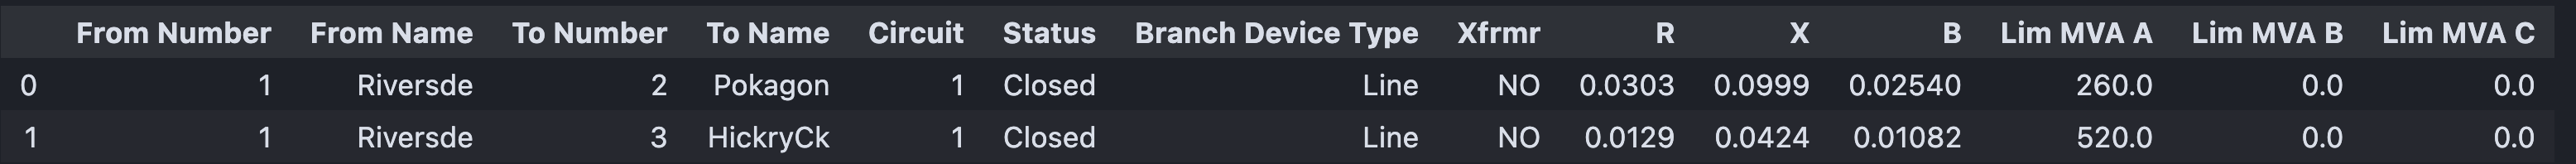
\includegraphics[width=0.95\textwidth]{image_7.png}
    \caption{Branch definitions imported from PowerWorld for the large-scale test instance.}
    \label{fig:branch-definitions}
\end{figure}

\begin{figure}[htbp]
    \centering
    \begin{minipage}[t]{0.55\textwidth}
        \centering
        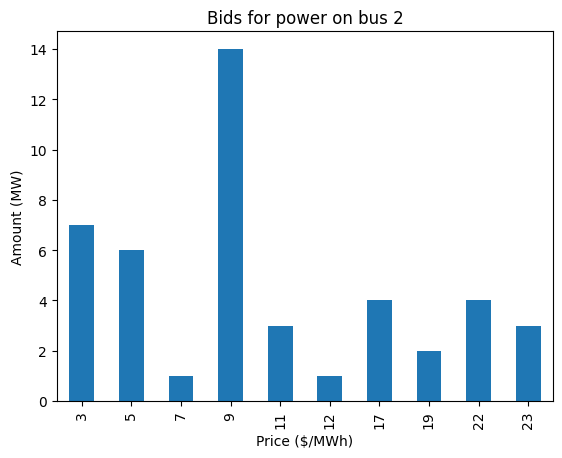
\includegraphics[width=0.9\linewidth,height=0.32\textheight,keepaspectratio]{image_4.png}

        \vspace{0.35em}
        \small Randomly generated bids for one bus.
    \end{minipage}\hfill
    \begin{minipage}[t]{0.45\textwidth}
        \centering
        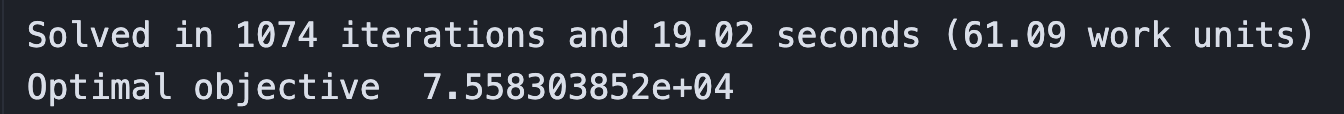
\includegraphics[width=\linewidth,height=0.16\textheight,keepaspectratio]{image_5.png}

        \vspace{0.35em}
        \small Final Gurobi solve-time summary.
    \end{minipage}
    \caption{Solution statistics on 118-bus model}
    \label{fig:computation-artifacts}
\end{figure}

\begin{figure}[htbp]
    \centering
    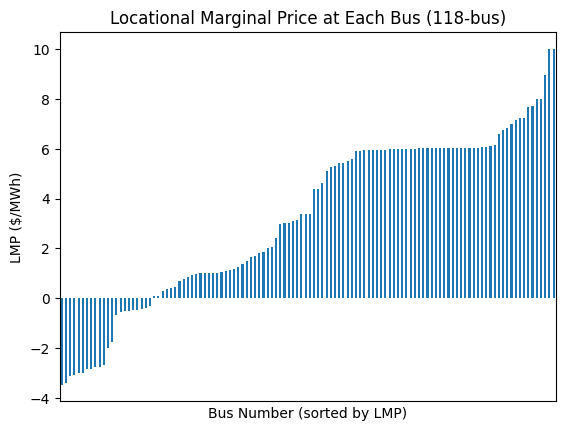
\includegraphics[width=0.74\textwidth]{image_9.png}
    \caption{Locational marginal prices across buses in the 118-bus instance, sorted by LMP.}
    \label{fig:lmp-distribution}
\end{figure}

\begin{figure}[htbp]
    \centering
    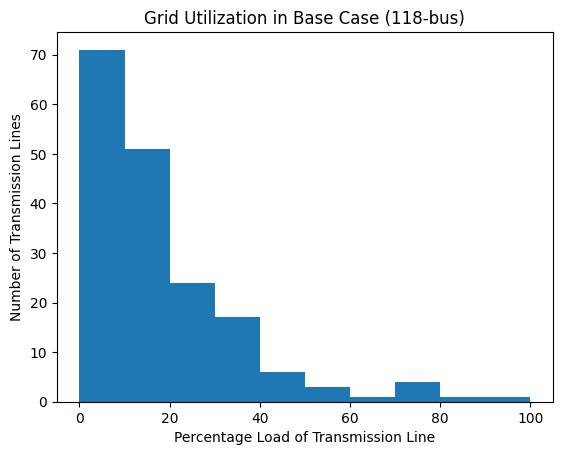
\includegraphics[width=0.72\textwidth]{image_6.png}
    \caption{Transmission-line utilization in the 118-bus base-case solution.}
    \label{fig:grid-utilization}
\end{figure}


\begin{figure}[htbp]
    \centering
    \begin{tikzpicture}
        \begin{axis}[
            width=0.88\textwidth,
            height=0.42\textheight,
            ymode=log,
            log basis y={10},
            symbolic x coords={24,30,39,57,118,300},
            xtick=data,
            enlarge x limits=0.12,
            xlabel={Network size (buses)},
            ylabel={Solve time (s, log scale)},
            ymajorgrids=true,
            yminorgrids=true,
            xmajorgrids=false,
            minor grid style={gray!15},
            major grid style={gray!30},
            tick label style={font=\scriptsize},
            x tick label style={font=\scriptsize},
            label style={font=\scriptsize},
            title style={font=\scriptsize},
            title={Observed solve time on our machine},
            mark options={scale=0.9},
        ]
            \addplot[
                very thick,
                blue,
                mark=*,
            ] coordinates {
                (24,0.06)
                (30,0.12)
                (39,0.12)
                (57,1.59)
                (118,21.33)
                (300,1953.45)
            };
        \end{axis}
    \end{tikzpicture}
    \caption{Observed solve times for increasingly large benchmark networks on our machine.}
    \label{fig:solve-time-scaling}
\end{figure}

\newpage

\section{Appendix: Data Previews}

\subsection{\texttt{branches.csv} preview}\label{app:branches-preview}
\textbf{Summary:} Branch definitions and parameters. Only Limit A applies for now.

\scriptsize
\begin{longtable}{@{}rrrrllcrrrr@{}}
\toprule
ID & From \# & To \# & Ckt & Status & Type & Xfrmr & $R$ & $X$ & $B$ & Limit A \\
\midrule
\endhead
1  & 1 & 2  & 1 & Closed & Line        & NO  & 0.00070 & 0.00123 & 0.00065 & 175.0 \\
2  & 1 & 5  & 1 & Closed & Line        & NO  & 0.02243 & 0.08490 & 0.02440 & 175.0 \\
3  & 2 & 4  & 1 & Closed & Line        & NO  & 0.03361 & 0.12730 & 0.03660 & 175.0 \\
4  & 2 & 6  & 1 & Closed & Line        & NO  & 0.05064 & 0.19201 & 0.05570 & 175.0 \\
5  & 3 & 1  & 1 & Closed & Line        & NO  & 0.05419 & 0.21114 & 0.06130 & 175.0 \\
6  & 3 & 9  & 1 & Closed & Line        & NO  & 0.03148 & 0.11921 & 0.03430 & 175.0 \\
7  & 4 & 9  & 1 & Closed & Line        & NO  & 0.02692 & 0.10779 & 0.02790 & 175.0 \\
8  & 5 & 10 & 1 & Closed & Transformer & YES & 0.02334 & 0.08837 & 0.02540 & 175.0 \\
9  & 7 & 8  & 1 & Closed & Line        & NO  & 0.01614 & 0.06103 & 0.01790 & 175.0 \\
10 & 8 & 9  & 1 & Closed & Line        & NO  & 0.04234 & 0.16482 & 0.04780 & 175.0 \\
\bottomrule
\end{longtable}
\normalsize

\subsection{\texttt{buses.csv} preview}
\textbf{Summary:} Bus-level voltage, angle, generation, and load data.

\scriptsize
\begin{longtable}{@{}rrrrrr@{}}
\toprule
Bus \# & Nom kV & PU Volt & Angle (deg) & Gen (\text{MW}) & Load (\text{MW}) \\
\midrule
\endhead
1  & 138.00 & 1.00000 & 0.00  & 35.85 & 0.00 \\
2  & 138.00 & 0.99783 & 0.01  & 67.00 & 97.00 \\
3  & 138.00 & 0.86395 & 10.75 & 0.00  & 90.00 \\
4  & 138.00 & 0.88721 & -0.42 & 0.00  & 74.00 \\
5  & 138.00 & 0.92693 & -0.22 & 0.00  & 71.00 \\
6  & 138.00 & 0.90837 & 0.39  & 0.00  & 68.00 \\
7  & 138.00 & 0.79668 & -0.58 & 64.00 & 62.00 \\
8  & 230.00 & 0.80581 & -0.87 & 0.00  & 85.00 \\
9  & 138.00 & 0.83528 & 4.98  & 0.00  & 175.00 \\
10 & 138.00 & 0.88216 & 3.72  & 0.00  & 100.00 \\
\bottomrule
\end{longtable}
\normalsize

\subsection{\texttt{ptdf.csv} preview}
\textbf{Summary:} PTDF/shift-factor matrix (rows: buses; columns: branches). Below is a small subset of columns.

\scriptsize
\begin{longtable}{@{}rrrrrr@{}}
\toprule
Bus \# & ETLR & WTLR & 1\,to\,2 & 3\,to\,1 & 1\,to\,5 \\
\midrule
\endhead
1  & 0.0000  & 0.0000  & 0.0000  & 0.0000  & 0.0000 \\
2  & -0.9962 & -1.4054 & -0.9946 & 0.0021  & -0.0033 \\
3  & 1.1629  & 1.0685  & -0.3619 & 0.4416  & -0.1965 \\
4  & -1.7811 & -1.6472 & -0.7309 & 0.1304  & -0.1387 \\
5  & -1.3303 & -1.0981 & -0.2290 & 0.0790  & -0.6920 \\
6  & -1.7217 & -1.9384 & -0.5453 & 0.1377  & -0.3170 \\
7  & -0.6366 & -0.9519 & -0.4875 & 0.2002  & -0.3124 \\
8  & -1.6366 & -1.0722 & -0.4875 & 0.2002  & -0.3124 \\
9  & -0.5991 & -0.5184 & -0.5076 & 0.2391  & -0.2533 \\
10 & -0.6740 & -0.7555 & -0.4673 & 0.1612  & -0.3714 \\
\bottomrule
\end{longtable}
\normalsize

\newpage
\section{References}
\begin{sloppypar}
\noindent
Sun, Junjie, and Leigh Tesfatsion. ``DC Optimal Power Flow Formulation and Solution Using QuadProgJ.'' \textit{ISU Economics Working Paper No. 06014}, revised 1 Mar.\ 2010, Iowa State University. \url{https://faculty.sites.iastate.edu/tesfatsi/archive/tesfatsi/DC-OPF.JSLT.pdf}. Accessed 5 Feb.\ 2026.
\end{sloppypar}

\noindent
ITI. ``models/electric-grid/physical/reference at master \textperiodcentered{} ITI/models.'' \textit{GitHub}. \url{https://github.com/ITI/models/tree/master/electric-grid/physical/reference}. Accessed 5 Feb.\ 2026.

\noindent
Southwest Power Pool. ``SPP Maps Frequently Asked Questions.'' \textit{SPP}. \url{https://www.spp.org/engineering/modeling/spp-maps-frequently-asked-questions/}. Accessed 5 Feb.\ 2026.

\noindent
Ma, Xingwang, David I. Sun, and Andy Ott. ``Implementation of the PJM Financial Transmission Rights Auction Market System.'' \textit{IEEE Power Engineering Society Summer Meeting}, 2002. \url{https://home.engineering.iastate.edu/~jdm/OldInfo/ArevaPJM2002.pdf}. Accessed 5 Feb.\ 2026.

\end{document}
